\documentclass[master.tex]{subfiles}
 
\newcommand{\meanxy}[1]{\left<#1\right>_{z,y}}
\newcommand{\Tflow}[0]{\overline{\Gamma}}

\begin{document}



\chapter{Effect of Polarization Equation Linearizations on tokamak edge turbulence}\label{sec:polarization_equation_evaluation}

\section{Introduction}
In both gyrokinetic and gyrofluid models the polarization equation plays a central role and the nonlinear nature is often approximated because of the large computational effort associated with the numerical schemes and the assumption that the amplitudes of turbulent fluctuations are much smaller than the background. This may hold for the core plasma but certainly not for the edge region where high background gradients are observed which lead to relatively high amplitude fluctuations if dense \textit{material} is transported from the core region of the separatrix into the \ac{SOL}. For instance the GYSELA polarization equation assumes a equilibrium density $n_0(r)$ where $r$ is to be identified with the $x$-direction \cite{GYSELACODE}. This comes close to linearization 3. The XGC1 code uses a similar approach \cite{XGC1Code}. The following results should give some insight on the effects of the different linearizations. It should be noted that this is not an extensive parameter study and considering the amount of parameters (>10) there could exist various other effects that are not represented by the particular parameters used in the following evaluation.

% The GENE code evaluates the non-linearity but the authors claim that it only has an effect if the electron Debye length $\lambda_{De}$ is comparable to the electron gyro radius $\rho_e$ which in a tokamak is not the case.

\section{Simulation Setup}

The evaluation of the linearizations is done on a 8x128x512 grid with $h_x$ and $h_y=1.0$ (low resolution) and on a 8x256x1024 grid with $h_x = h_y=0.5$ (low resolution). Two parameter sets are tested (for both resolutions). Both sets share the same parameters expect for the perpendicular hyperviscosity $\nu_\perp$:
\begin{itemize}
    \item $\Delta t$: 0.01
    \item $\hat{c}$: 5.0
    \item $\hat{\epsilon}$: 27000.0
    \item $\mathcal{K}_0$: 0.02
    \item $magnetic Shear$: 1.2
    \item $\delta$: 0.015
    \item $\nu_{\parallel}$: 0.2
    \item core Density: 1.2
    \item edge Density: 0.13
\end{itemize}
For the first parameter set $\nu_{\perp} = 0.64|0.04$ (low|high) and for the second set $\nu_{\perp} = 0.96|0.06$. The change of $\nu_\perp$ for the low and high resolution was chosen this way because the term is used to cut off high frequency modes in perpendicular direction. But at a finer resolution in that direction it is not necessary anymore to cut off these modes. Since we are using the fourth derivative in each direction for each direction we get a factor of 4 (in the Fourier-space) and because of that reduce $\nu_\perp$ by $\frac{1}{16} = \frac{1}{4\cdot4}$ to $\nu_\perp = 0.04|0.06$. $\nu_\parallel$ stays untouched since we didn't change the resolution in z-direction \footnote{It should be noted though that through magnetic shearing there could actually be an effect from higher perpendicular resolution on the parallel direction} \newline
The simulation is run on \ac{TV} node using the GPU implementations of the \ac{SOR}-solver and gyroaveraging operator. Both versions are run for 150,000 iterations and full data output is created every 15,000 iterations. Combined qunatities (Turbulent Flow, Parallel Kinetic Energy...) are recorded every 20 iterations.


\section{Equilibrium State}
At first the simulation develops strong turbulence and high fluctuations which result in an outburst of "material" (i. e. the total density decreases). Afterwards the simulation approaches a steady state where the state variables only vary little and a typical energy cascade forms. This equilibrium behavior can be seen by looking for instance at temporal evolution of the parallel kinetic energy (\autoref{sec:polar_parallel_velocities}) or the total density both restricted to the core and \ac{SOL} plasma (in/out separatrix) . The data suggests that a stable regime is reached after about 100,000 iterations\footnote{This is not the case for each and every presented simulation but it is at least fairly stable after 100,000 iterations. Future studies should increase the iterations run to at least 250,000 and chose a later point in time.}. The idea now is to compare mean values over the simulation time where a equilibrium state has been reached. 

% \begin{figure}[!hbtp]
%     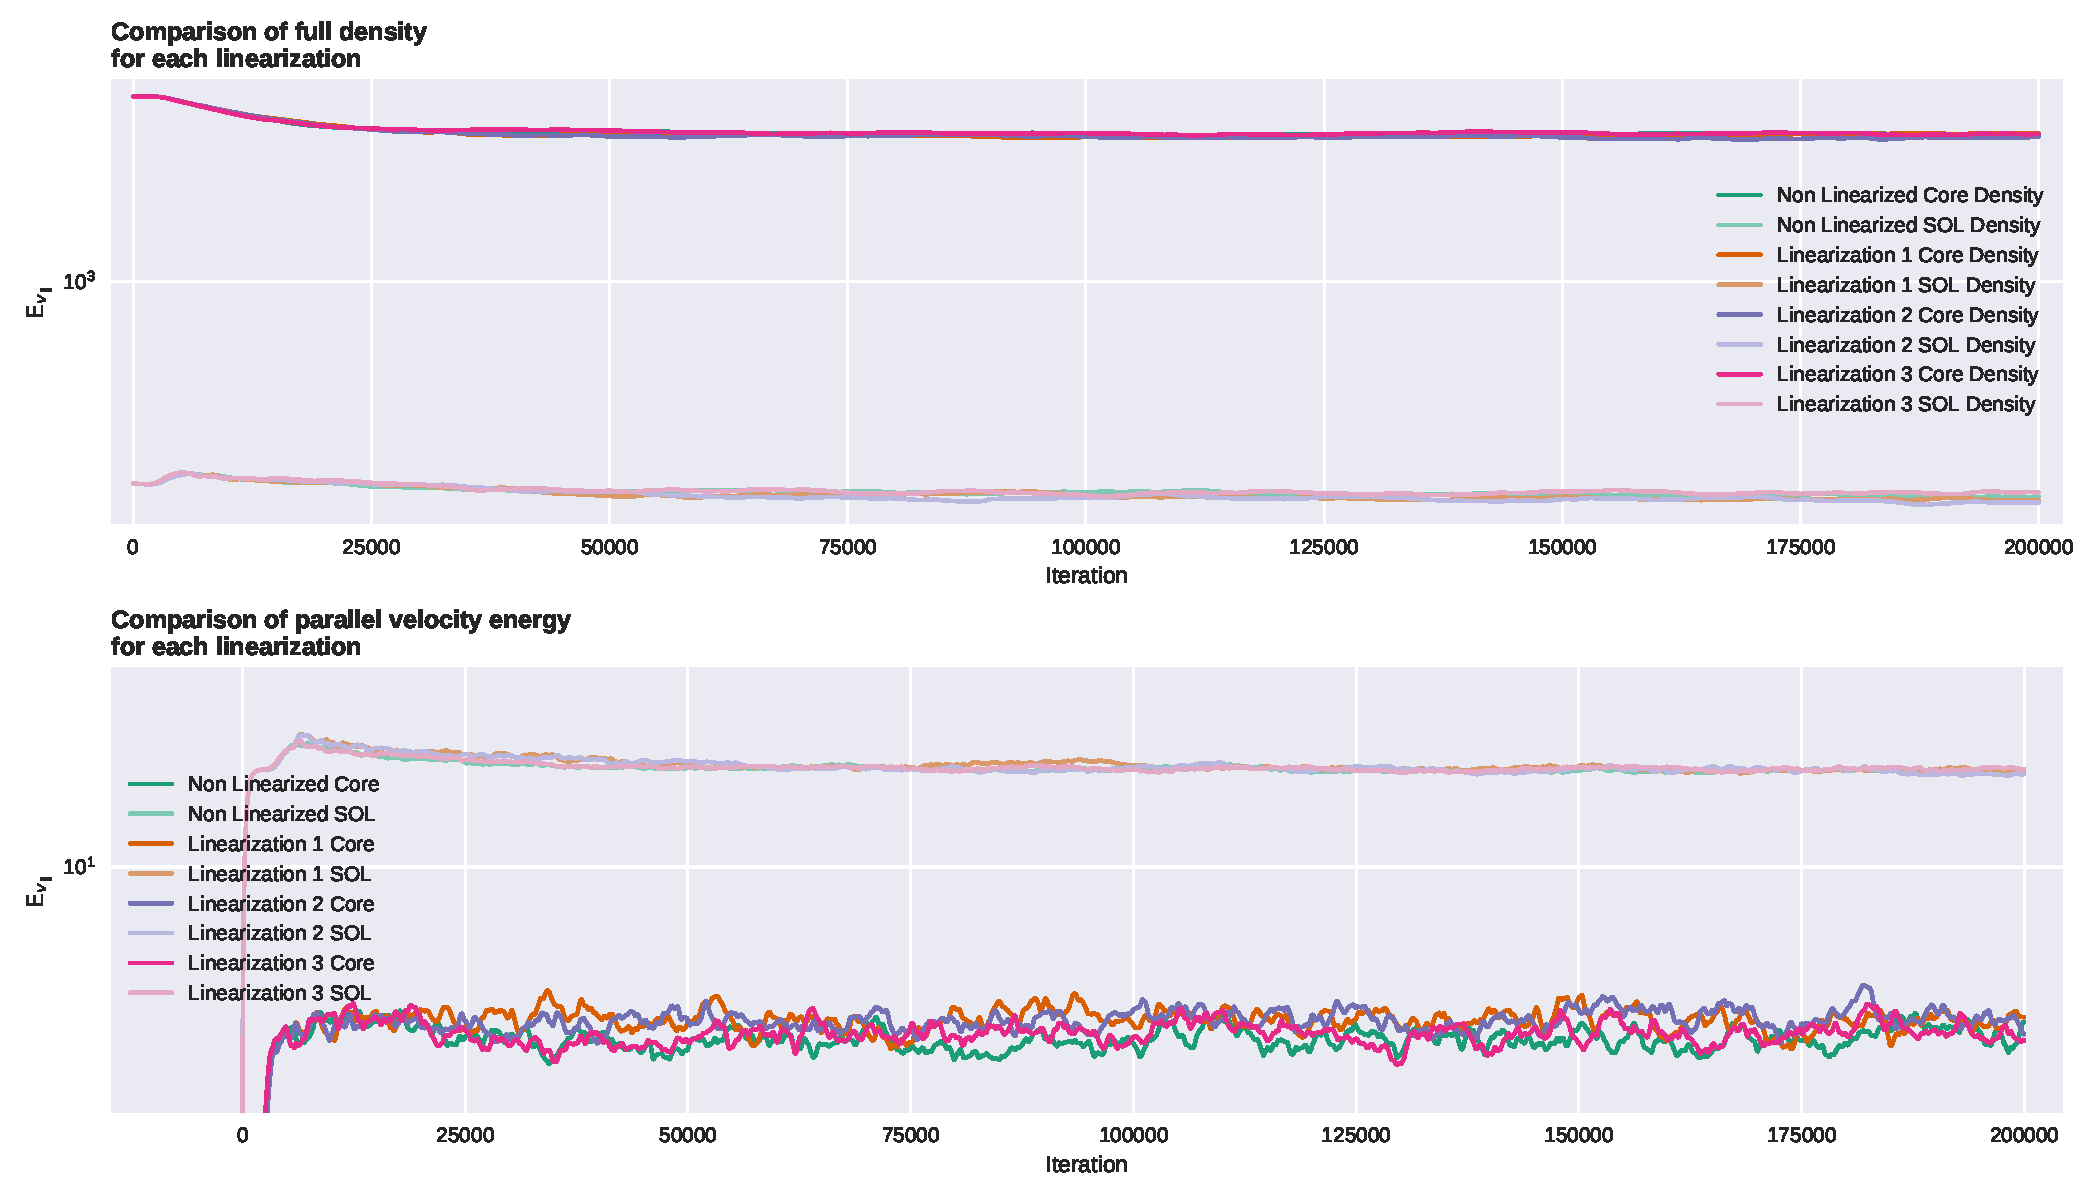
\includegraphics[width=\linewidth]{pdfs/equilibrium_state_low.pdf}
%     \caption{Temporal evolution of ($E_n$ \autoref{sec:fluid-dynamics}) and the parallel kinetic energy (see \autoref{sec:polar_parallel_velocities}) both restricted to Core and \ac{SOL} region. After 80,000 iterations a steady state is reached.}
% \end{figure}


\begin{blockquote}
    The errors attached to the mean values are calculated via the standard derivation but do not represent the error of multiple simulations or the response to disturbed input parameters but rather give an idea about the size of fluctuations in the equilibrium state.
\end{blockquote}
    
\section{Evaluation}
To compare the different linearizations defined in \autoref{sec:polarization-linearizations} the mean turbulent flow in the steady state regime is compared for the Core and \ac{SOL} plasma. Further on the zonal potential  $\meanxy{\phi_e}$, the zonal flow ($\partial_x \meanxy{\phi_e}$), the vorticity ($\partial_{xx}\meanxy{\phi_e}$) and the zonal turbulent flux ($\left<\Gamma^*\right>_{z,y}$\footnote{In this case $\Tilde{n}_s$ is calculated using the intial density profile: $\Tilde{n}_s = n_s - n_0$.}) are compared and finally also the parallel kinetic energy is discussed. The evaluation methods are now described for the first parameter set at low resolution and will be reused for the other sets.


\section{Turbulent Flow}
The turbulent flow is calculated as it is defined in \autoref{sec:simulation_quantities}. The turbulent flows (Core/\ac{SOL}) for the whole simulation are displayed in \autoref{fig:turbulent-flow-low} on a semi logarithmic grid. From this figure one can already see that there is no apparent difference for the turbulent flows in regard to the linearizations for the first parameter set.
\begin{figure}[!htbp]
    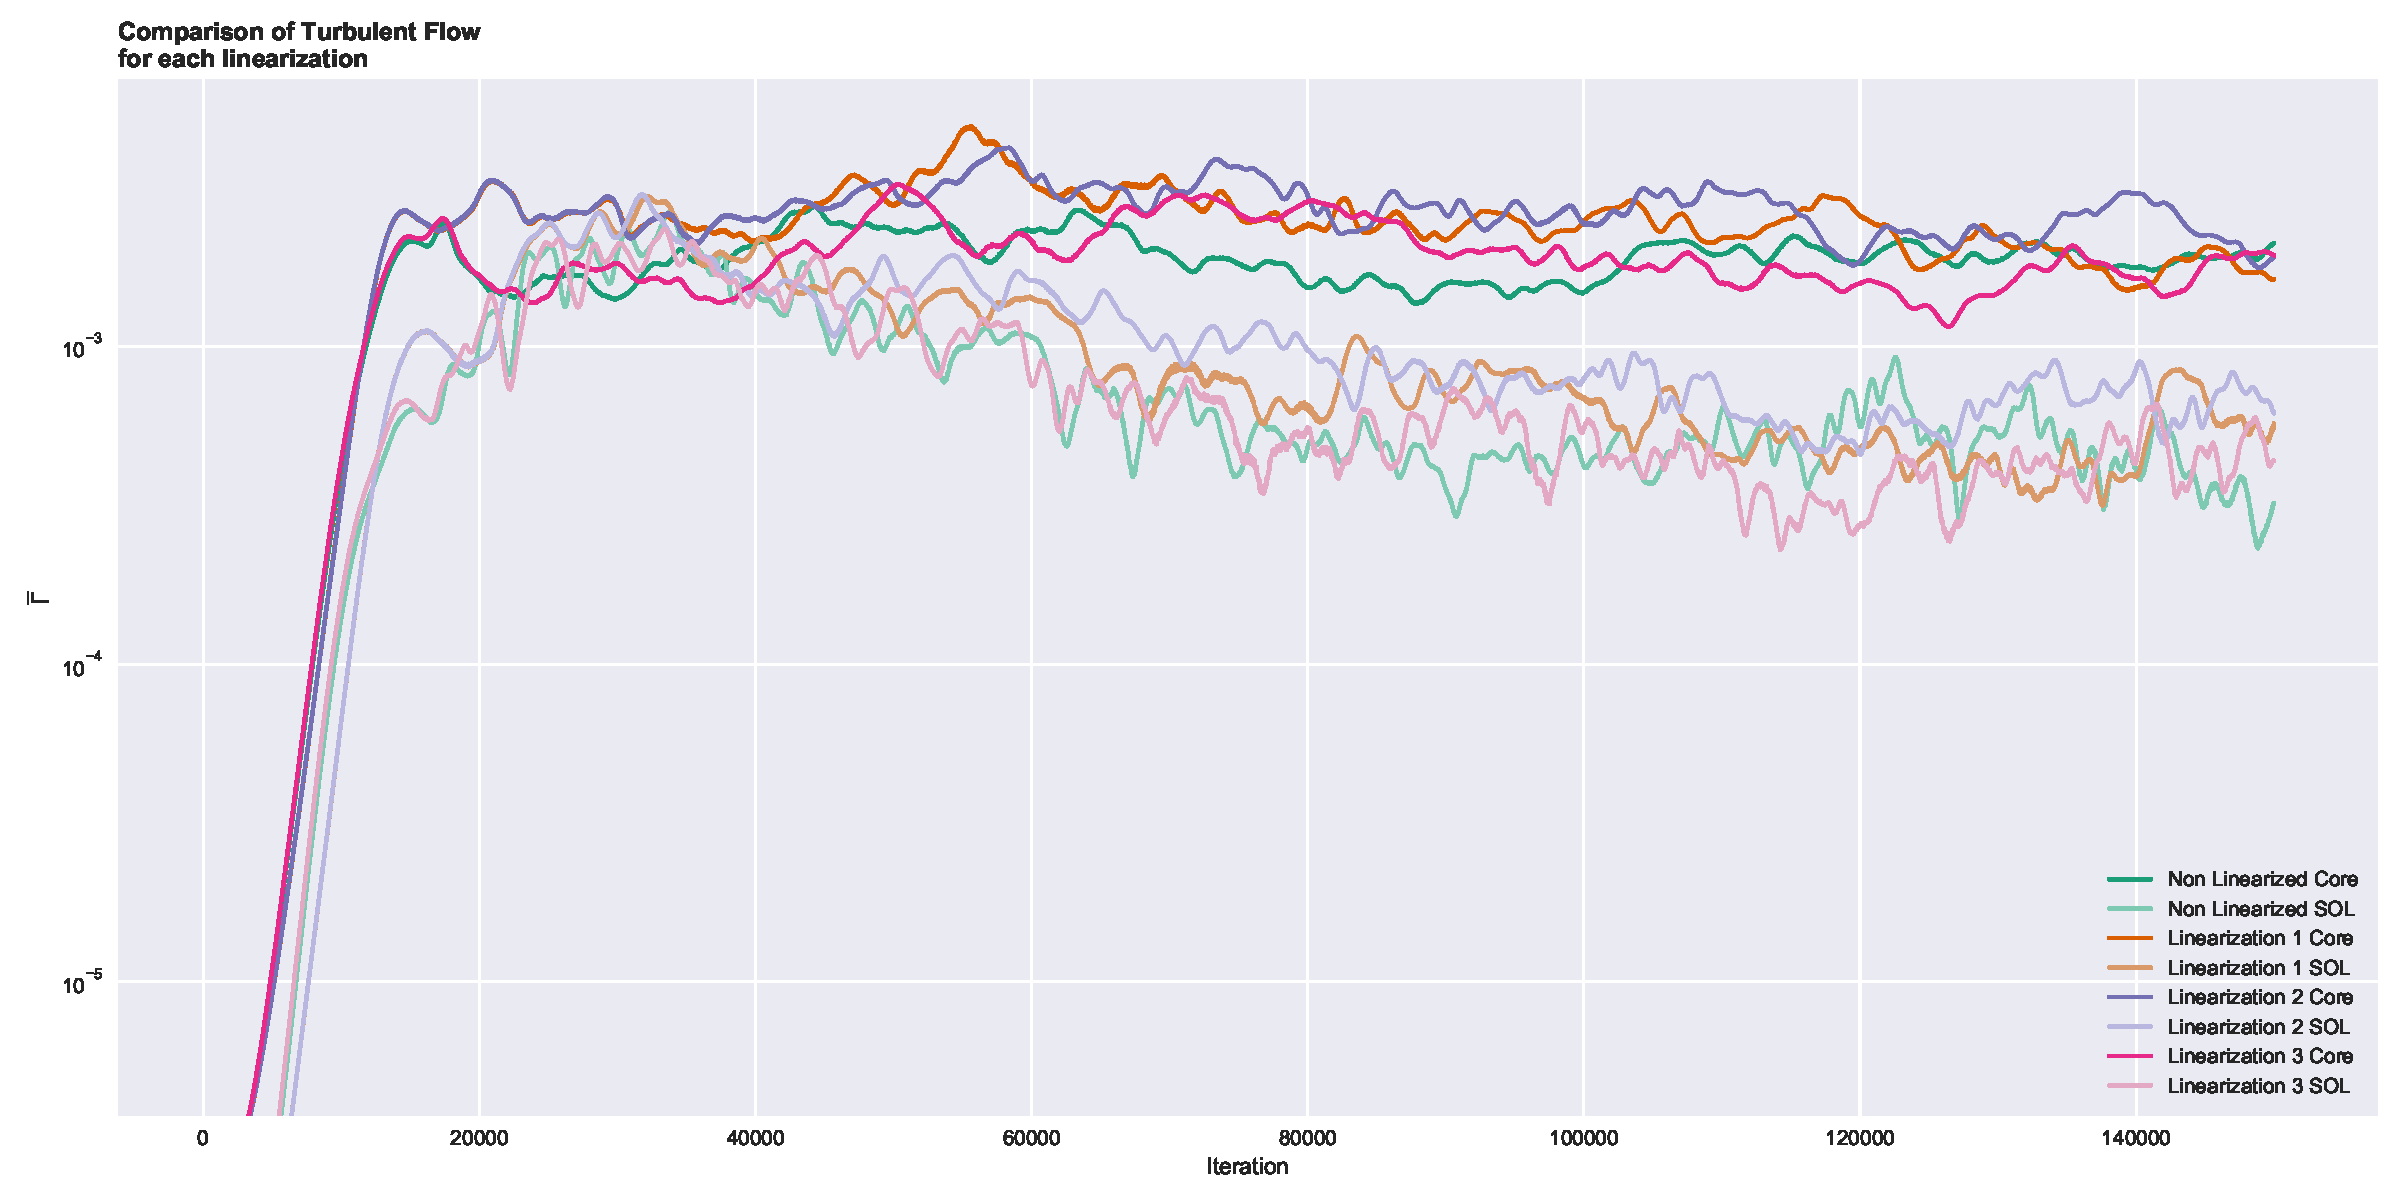
\includegraphics[width=\linewidth]{pdfs/0-2_0-64/turbulent-flow-time.pdf}
    \caption{Turbulent flow split into Core and \ac{SOL} region for each linearization. The lighter colors represent the \ac{SOL} parts.}
    \label{fig:turbulent-flow-low}
\end{figure}
\autoref{fig:turbulent-flow-low-means} shows the mean value of $\Tflow_{Core}$ and $\Tflow_{SOL}$ from 100,000 to 150,000 iterations. There may be a small indication that $\Tflow_{Core}$ is a little higher for the constant background (local model) linearizations especially when compared to the third linearization. 



\begin{figure}[!htbp]
    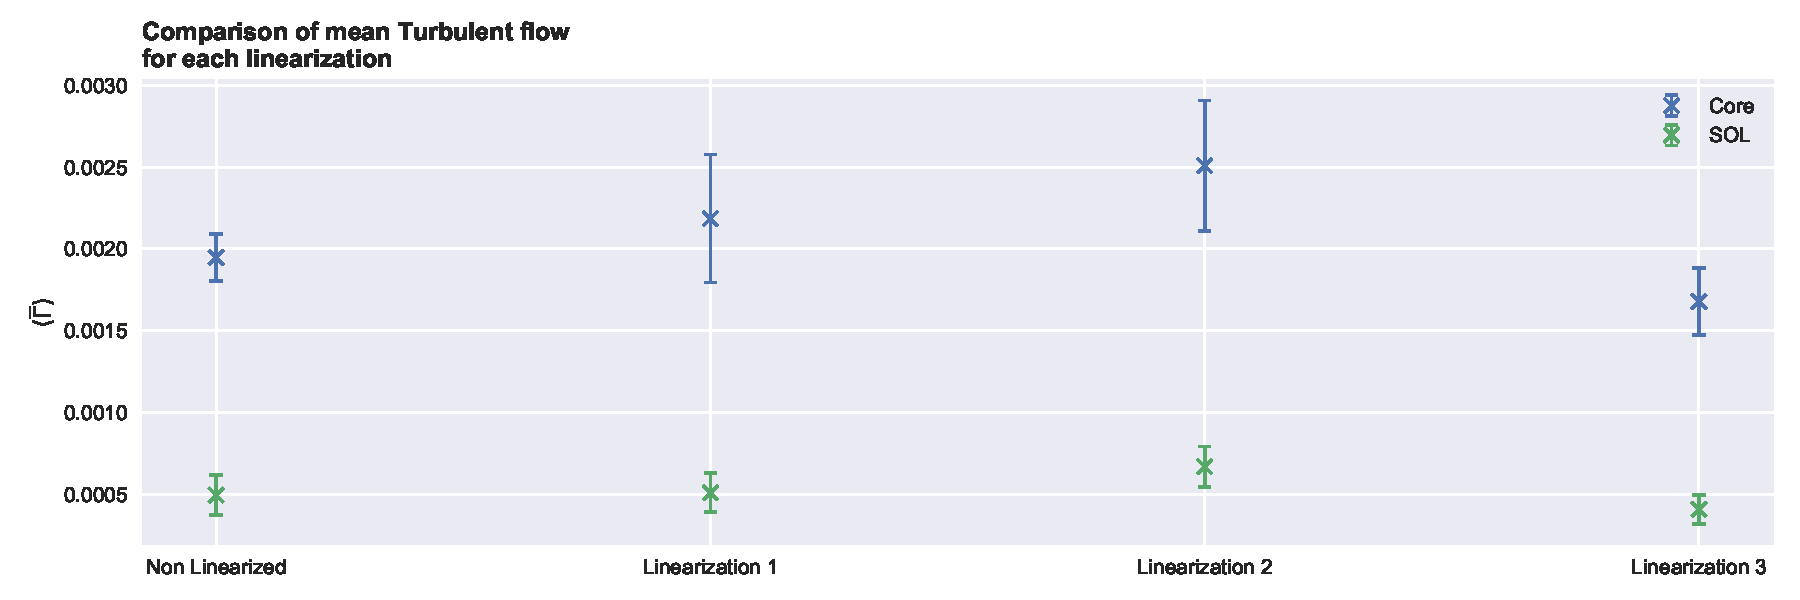
\includegraphics[width=\linewidth]{pdfs/0-2_0-64/turbulent-flows-mean-100000.pdf}
    \caption{Mean values of $\Tflow$ after 100,000 iterations.}
    \label{fig:turbulent-flow-low-means}
\end{figure}

\section{Zonal Profiles}

The same procedure of the previous section is applied to the zonal potential, zonal flow, zonal vorticity and the turbulent flux. The results are shown in \autoref{fig:zonal-potential-low-all}.\\
They form two groups: The non linearized model and the third linearization share distinct features as well as the first and the second (mainly in the \ac{SOL} region). This can mainly be seen by looking at the Turbulent Flux (fourth figure) where the third linearizations fits very good to the non linearized version. Also the Zonal Flows fit together in the \ac{SOL} region. Since the linearization specifically targets the gradient of the densities which is the strongest close to the Core plasma, differences between the linearizations and the non linearized model are observed there. Also in the \ac{SOL} region where the background density is small compared to the fluctuations the linearizations have a strong impact whereas in the \textit{middle} region around the separatrix there are less differences visible.

\begin{figure}[!htbp]
    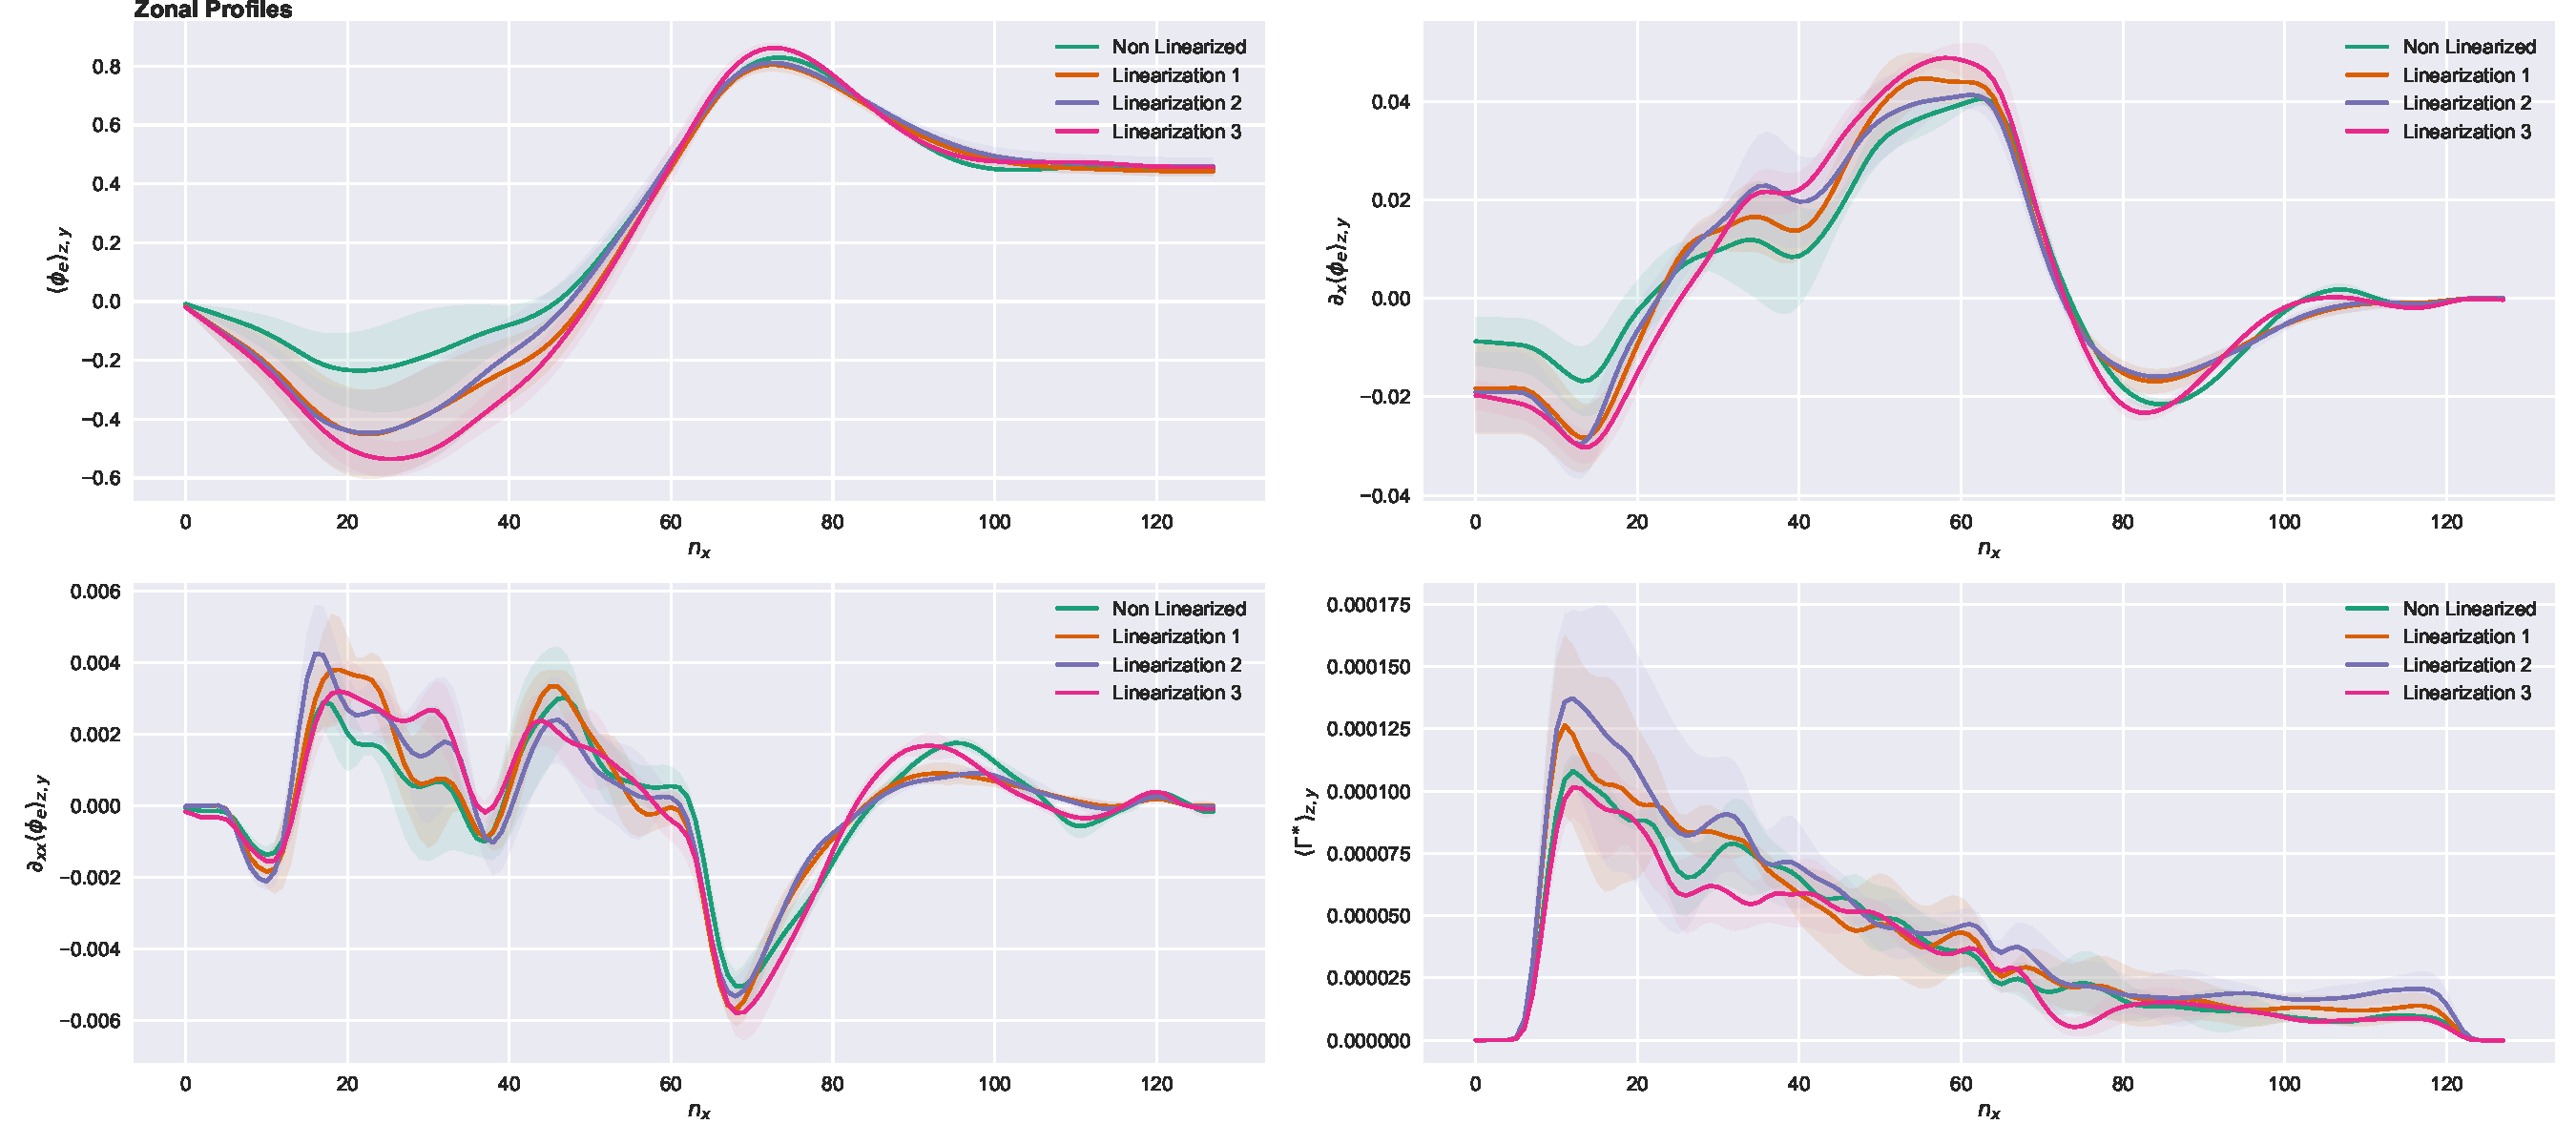
\includegraphics[width=\linewidth]{pdfs/0-2_0-64/zonal-profiles-100000.pdf}
    \caption{Mean values of Zonal Potential, Zonal Flow and Zonal Flow Potential of iteration 100,000-150,000. The shaded areas show fluctuations for each case.}
    \label{fig:zonal-potential-low-all}
\end{figure}

\section{Parallel Kinetic Energy $E_{v\parallel}$}\label{sec:polar_parallel_velocities}

To \textit{measure} the influence in the parallel direction it might be helpful to look at the $E_{v\parallel}$ as it is defined in \autoref{sec:fluid-dynamics}.\newline
As in the previous chapters the integration will be restricted to either Core or the \ac{SOL} region. The mean values are shown in \autoref{fig:velocity-energy-low-mean}. This quantity nicely shows the formation of the two groups. But the differences are only visible in the Core region. Since $E_{v\parallel}$ is heavily influenced by the boundary conditions in the \ac{SOL} effects from the linearizations might be suppressed.

\begin{figure}[!htbp]
    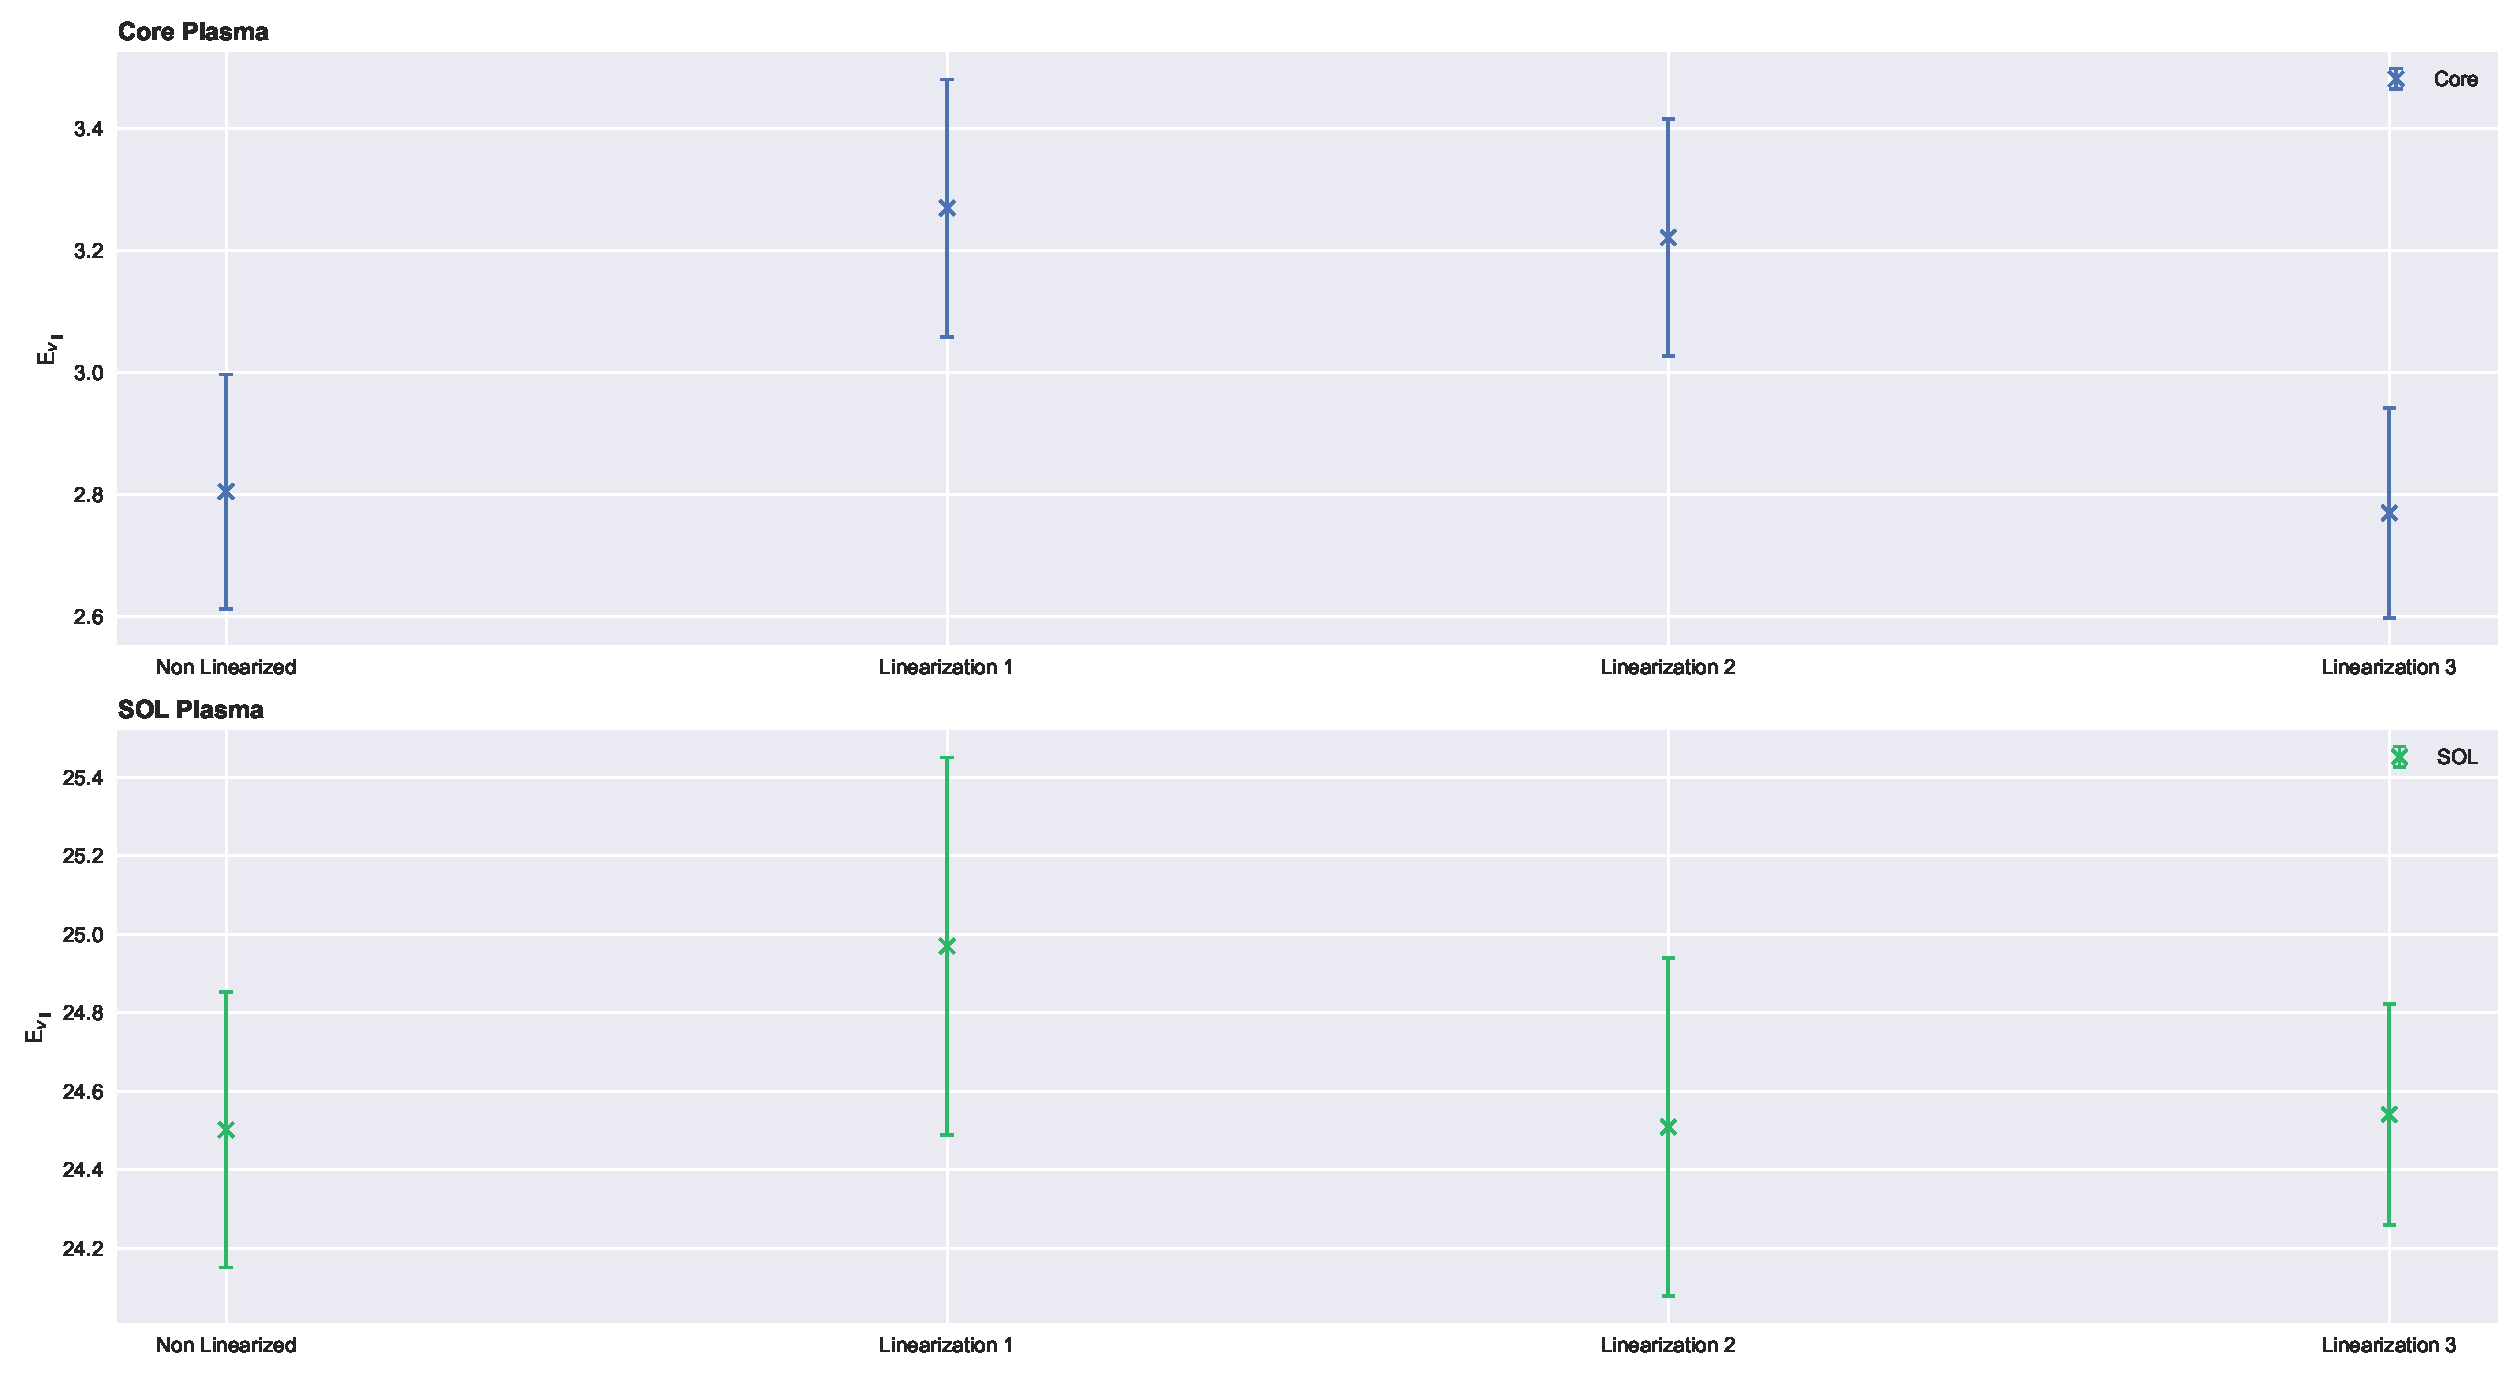
\includegraphics[width=\linewidth]{pdfs/velocity-energy-low-means.pdf}
    \caption{Mean of Parallel Kinetic Energy from 100,000 to 150,000 iterations}
    \label{fig:velocity-energy-low-mean}
\end{figure}


\section{High resultion Data 1\textsuperscript{st} parameter set}
The data from the first data set at a higher resolution is presented in \autoref{fig:high-resoultion-set-1}. At the higher resolution the differences for the Zonal Profiles in the Core region are generally greater and here there are also great differences between the linearized versions the non linearized ones but closer to the \ac{SOL} these differences become less and less. The formation of the two groups is not generally visible anymore hinting that density fluctuations in $y$-direction now play a greater role compared to the lower resolution simulation. The Turbulent Flow and the Turbulent Flux in the \ac{SOL} region especially at the very end are almost double the size for the higher resolution set. The parallel kinetic energy shows the formation of the two groups again but this time stronger. It is clearly visible in the \ac{SOL} region and Interestingly the picture for the Core region is inverted compared to the lower resolution. It might be that for the first group the higher resolution localizes more of this energy in the Core region compared to the lower resolution set. The effect seems to be connected to the density gradient in $x$-direction since it is much stronger for the first group.


\begin{figure}[!hbtp]
    \textbf{Zonal Profiles, mean Turbulent flows and Parallel Kinetic Energies}\par\medskip
    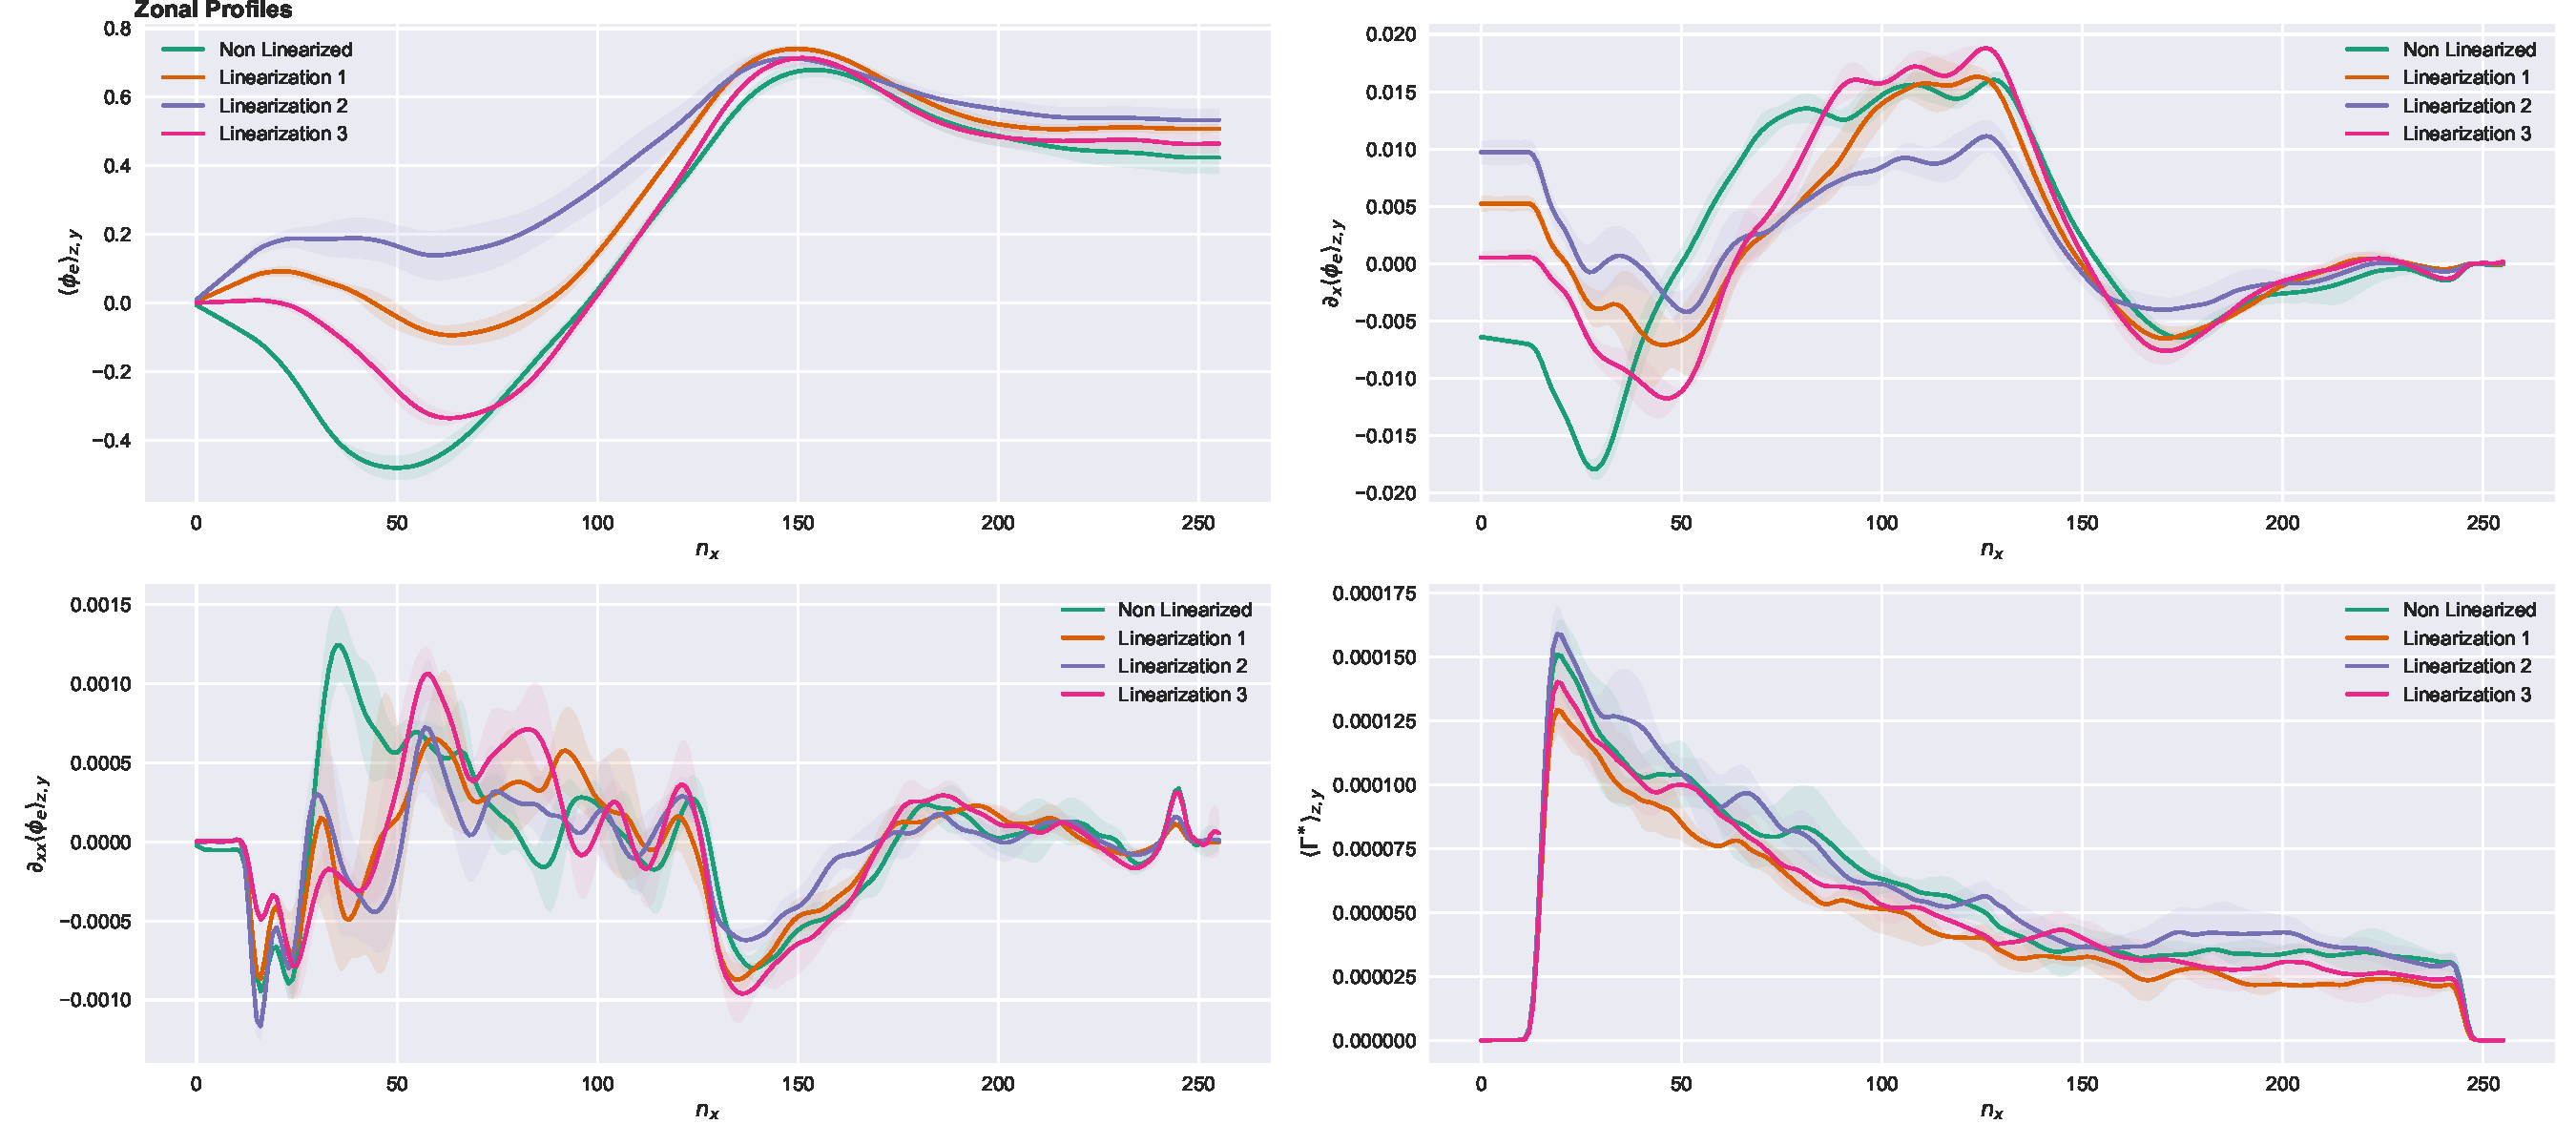
\includegraphics[width=\linewidth]{pdfs/0-2_0-04/zonal-profiles-100000.pdf}
    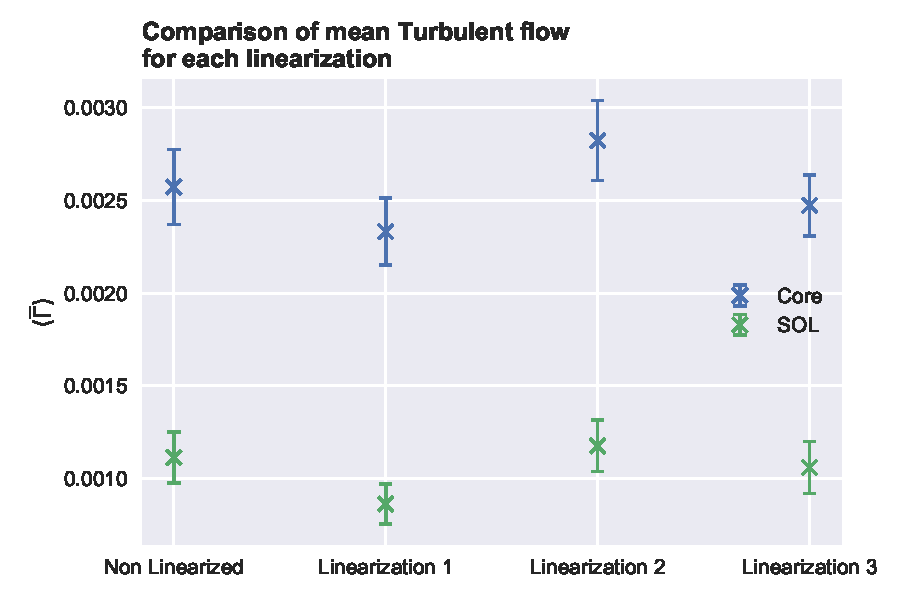
\includegraphics[width=0.5\linewidth]{pdfs/0-2_0-04/turbulent-flow-means.pdf}
    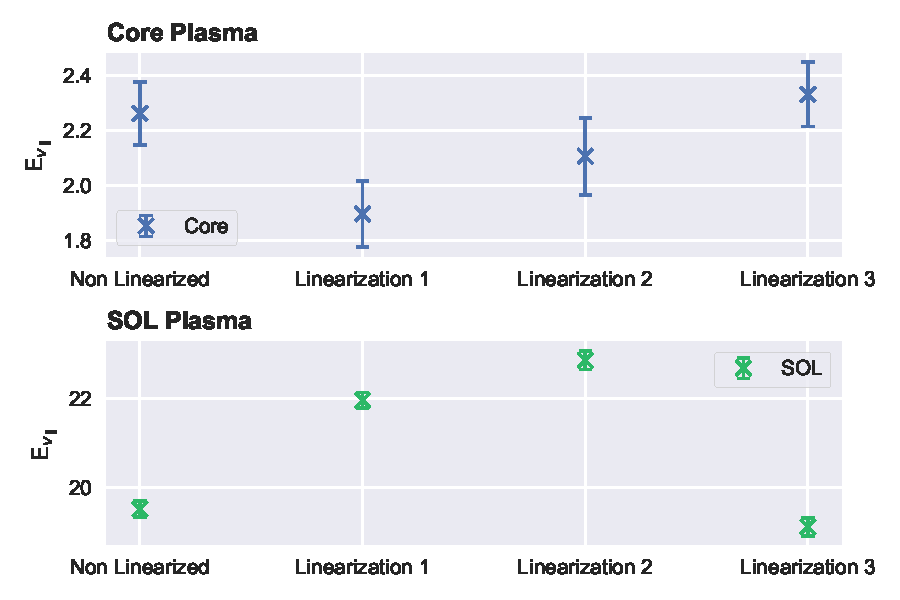
\includegraphics[width=0.5\linewidth]{pdfs/0-2_0-04/velocity-menas-100000.pdf}
    \caption{Zonal Profiles, mean Turbulent Flows and mean parallel Kinetic Energies for the 1\textsuperscript{nd} parameter set at high resolution $h_x = h_y = 0.5$. The mean values are taken from iteration 100,000 to 150,000.}
    \label{fig:high-resoultion-set-1}
\end{figure}



\section{2\textsuperscript{nd} Parameter Set}
The second parameter set only changes for the perpendicular hyperviscosity which is increased to $v_\perp = 0.96 | 0.06$ for $h_x=h_y=1.0|0.5$ respectively.

\subsubsection{Low Resolution (8x128x512 $h_x=h_y=1.0$)}

First the results of the low resolution set are presented in \autoref{fig:low-resoultion-set-2}.

\begin{figure}[!hbtp]
    \textbf{Zonal Profiles, mean Turbulent flows and Parallel Kinetic Energies}\par\medskip
    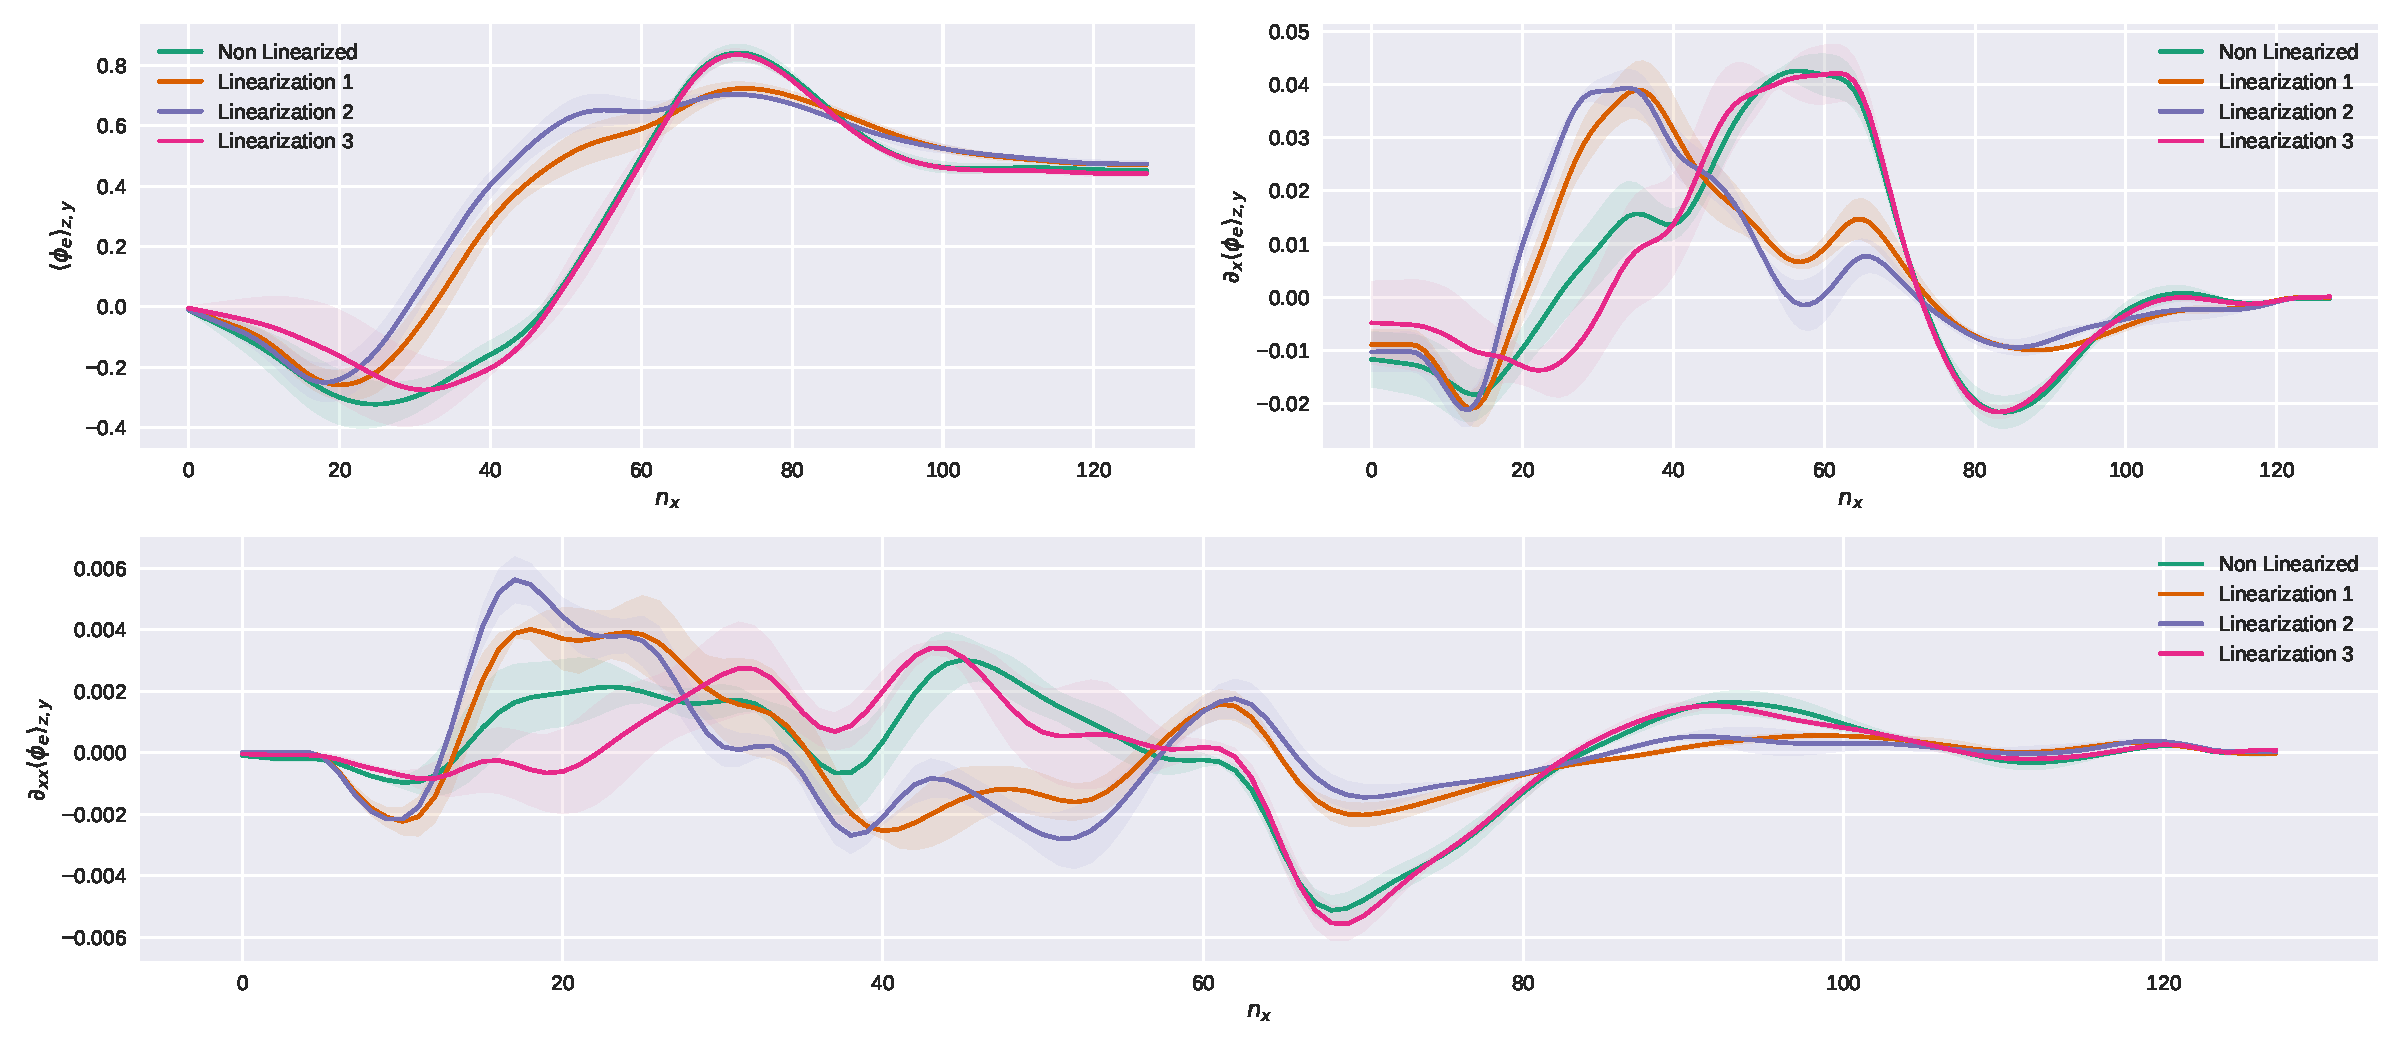
\includegraphics[width=\linewidth]{pdfs/0-2_0-96/zonal_profiles_100000.pdf}
    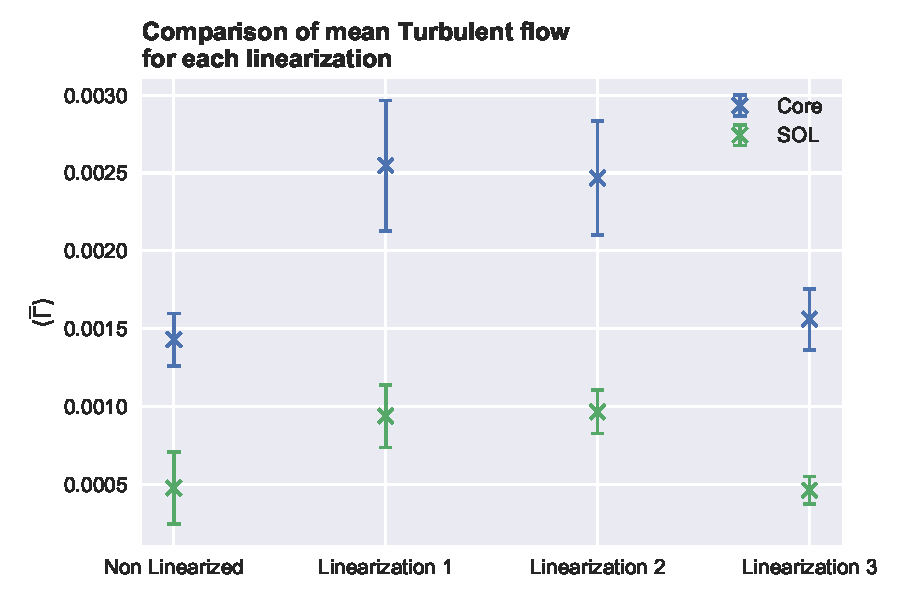
\includegraphics[width=0.5\linewidth]{pdfs/0-2_0-96/turbulent_flow_means_100000.pdf}
    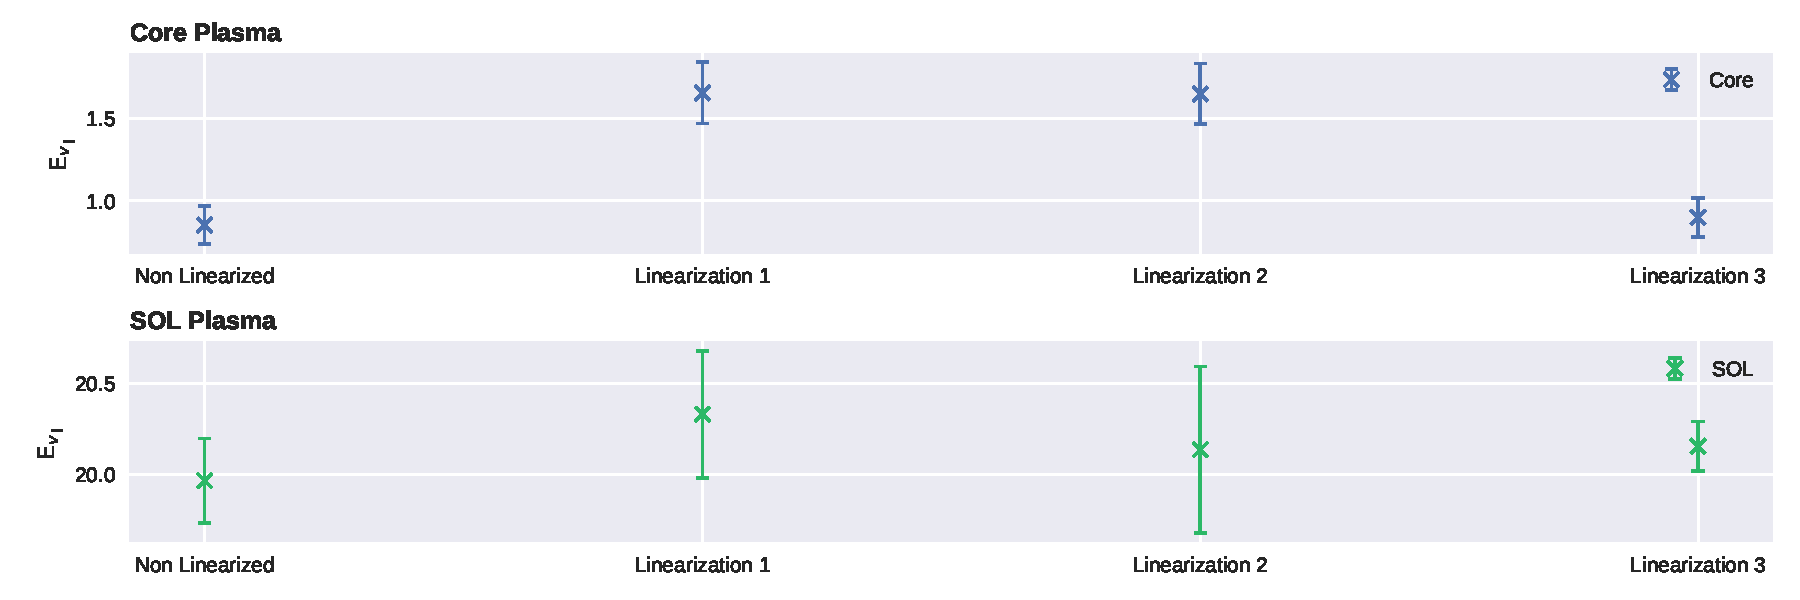
\includegraphics[width=0.5\linewidth]{pdfs/0-2_0-96/parallelvelocity_mean_100000.pdf}
    \caption{Zonal Profiles, mean Turbulent Flows and mean parallel Kinetic Energies for the 2\textsuperscript{nd} parameter set at low resolution $h_x = h_y = 1.0$. The mean values are taken from iteration 100,000 to 150,000.}
    \label{fig:low-resoultion-set-2}
\end{figure}



The two groups from the previous section are formed again, but this time more differences between them are visible. For instance the maximum zonal flow is achieved much close to the separatrix for the first group.\newline
Also for the turbulent flow and the parallel kinetic energies the two groups are visible again. As in the previous section the second group produces higher turbulent flows and parallel kinetic energies at the lower resolution.\newline
For this parameter set the differences between the linearizations are generally more significant and for example the $\left< \overline{\Gamma} \right>$ in the Core region for the non linearized polarization equation is double the magnitude of the linearization one. As the only difference to the first parameter set is $\nu_\perp$ one can see that this parameter has different effects on the linearizations.\newline
Also for these parameters the turbulent flux is much smaller for the first group. The higher $\nu_\perp$ seems to have a much stronger influence on the first group according to the values for the turbulent flow if one compares this to the lower resolution case of the first parameter set.


\subsubsection{High Resoltion (8x256x1024 $h_x = h_y = 0.5$)}

The high resolution data for the 2\textsuperscript{nd} parameter set is persented in \autoref{fig:high-resoultion-set-2}

\begin{figure}[!hbtp]
    \textbf{Zonal Profiles, mean Turbulent flows and Parallel Kinetic Energies}\par\medskip
    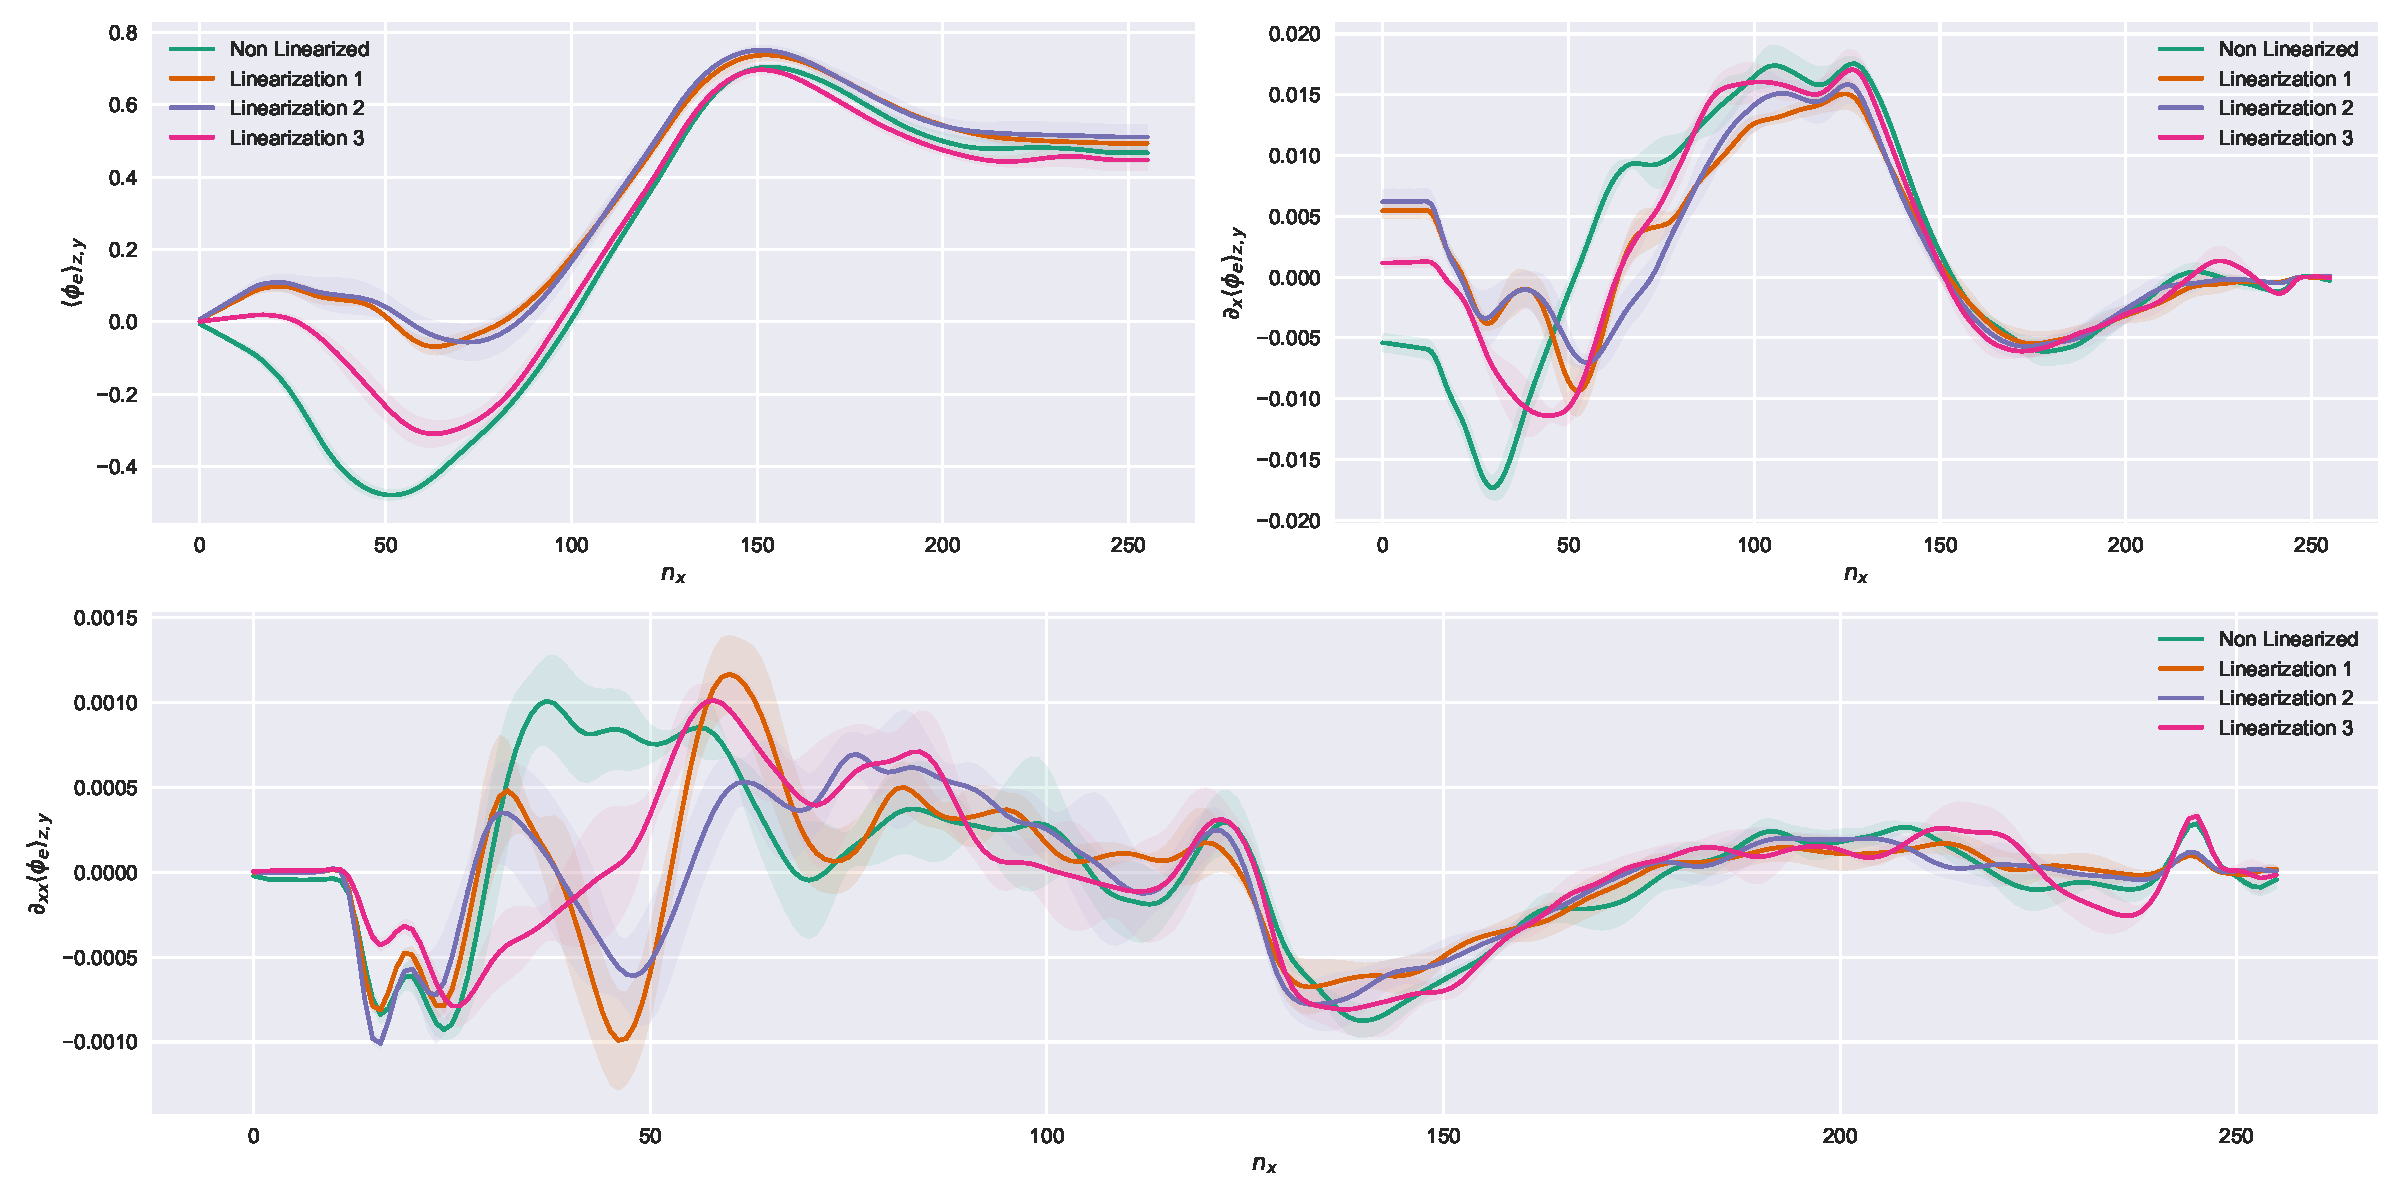
\includegraphics[width=\linewidth]{pdfs/0-2_0-06/zonal_profiles_100000.pdf}
    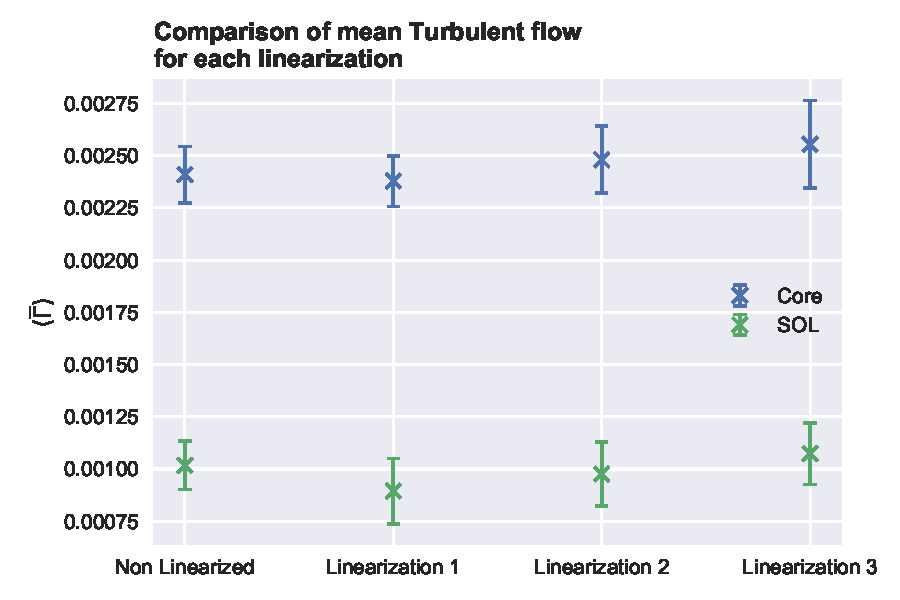
\includegraphics[width=0.5\linewidth]{pdfs/0-2_0-06/turbulent_flow_means_100000.pdf}
    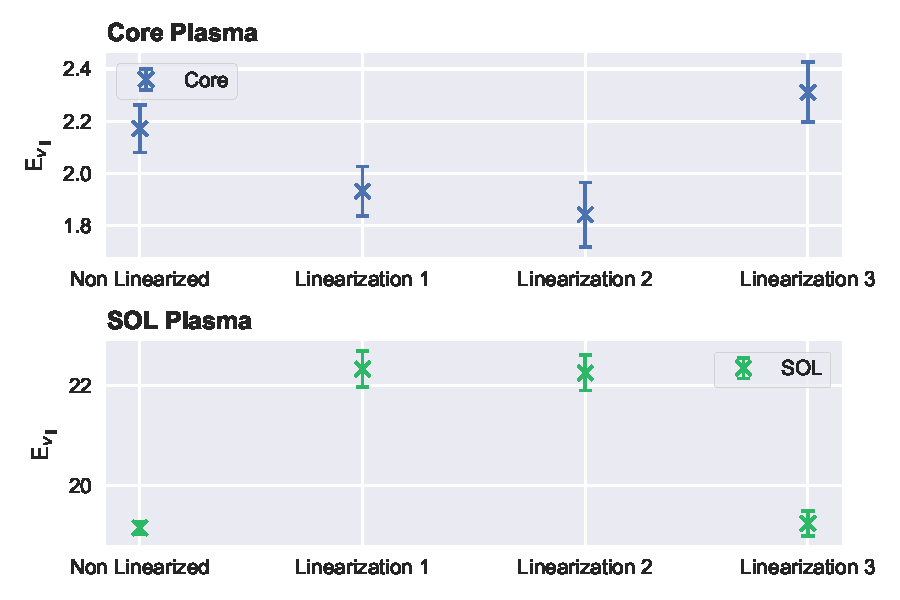
\includegraphics[width=0.5\linewidth]{pdfs/0-2_0-06/parallel_energies_100000.pdf}
    \caption{Zonal Profiles, mean Turbulent Flows and mean parallel Kinetic Energies for the 2\textsuperscript{nd} parameter set at higher resolution $h_x = h_y = 0.5$. The mean values are taken from iteration 100,000 to 150,000.}
    \label{fig:high-resoultion-set-2}
\end{figure}

At the higher resolution the great differences between the first and second group seen in the Zonal Flow profile vanish again. Also the mean Turbulent Flow and Turbulent Flux profile now are closer together for each linearization. In general both high resolution sets produce similar results. This hints that the viscosity scaling is probably wrong for higher viscosities and the 2\textsuperscript{nd} parameter set at lower resolution should be treated with caution.  



\section{Numerical stability}
Not thoroughly measured was the stability of the simulation but still some information will be presented here. For example if one increases the magnetic curvature to 0.05 for the lower resolution grid (leading to stronger turbulence) only the non linearized model is numerical stable. One has to deal with high gradients at the boundaries which seem to be a greater problem for the linearized models. 
Furthermore if the resolution is increased the $\Delta t$ has to be decreased but the non linearized model is still stable for higher $\Delta t$'s whereas the linearizations are much more sensitive to an increase of the resolution and need smaller $\Delta t$'s. It seems that the \ac{CFL} number is higher for the linearized models.

\section{Conclusion}

In this chapter the effects of the different linearizations where evaluated on a 3-dimensional grid representing the edge area of a tokamak using the Isothermal 3D Full-F Gyrofluid Model presented in \autoref{sec:isothermalequations}. The simulation was run for two different parameter sets that only differed in $\nu_\perp$ each at two different resolutions $h_x=h_y=1.0|0.5$.
As is expectable the polarization equation versions form two groups. The first group consists out of the non linearized version and the third linearization. Both of them still consider the background density gradient in $x$-direction where the second group (first and second linearization) both assume no gradient in the background density. This effect is mostly seen at the simulation boundaries where artificial strong gradients exist, but also in the core region. Especially the zonal profiles show greater deviations in the core region than in the SOL region.\newline
The second parameter set shows some unusual behavior and strong differences between the linearizations at the lower resolution which uses a very high perpendicular hyperviscosity. Because of that this data set should only be considered with caution.\newline
The low resolution sets are generally questionable since the viscosities need to be chosen very high to achieve a stable simulation. Because of that further on the discussion only relates to the higher resolution parameter sets.\newline
At this resolution the differences in the zonal profiles are mostly visible in the Core region. Here there are also great differences between the non-linearized and the third version. This hints that in that region fluctuations in $y$-direction are of the size of the background whereas it does not seem to play major role in the \ac{SOL} region. Generally the zonal profiles look very much the same beyond the separatrix (expect for the very boundary where numerical artifacts play a major role). The turbulent flows are of the same order for each linearization. This can not be said for the parallel kinetic energy. Here it looks like the first group concentrates more of $E_{v\parallel}$ in the Core region and the second group more in the \ac{SOL} region. In this region the effects of the limiter boundary conditions play a major role since they have a strong effect on $v_{\parallel}$. These differences suggest that the constant background linearizations should be used with caution when considering such boundary conditions.\newline
There are no major differences visible in the Turbulent flux. The structure as well as the absolute values are of the same size for each linearization as well as for both parameter sets but are a little higher for the non linearized version and the second linearization at the lower perpendicular hyperviscosity. But this effect is very small compared to the fluctuations.\newline
In the end there are differences visible between the linearizations and even the fluctuations in $y$-direction have an impact.





\end{document}